\documentclass[12pt]{article}
\usepackage[left=1cm, right=1cm, top=2cm,bottom=1.5cm]{geometry} 

\usepackage[parfill]{parskip}
\usepackage[utf8]{inputenc}
\usepackage[T2A]{fontenc}
\usepackage[russian]{babel}
\usepackage{enumitem}
\usepackage[normalem]{ulem}
\usepackage{amsfonts, amsmath, amsthm, amssymb, mathtools,xcolor}
\usepackage{blkarray}

\usepackage{tabularx}
\usepackage{hhline}

\usepackage{accents}
\usepackage{fancyhdr}
\pagestyle{fancy}
\renewcommand{\headrulewidth}{1.5pt}
\renewcommand{\footrulewidth}{1pt}

\usepackage{graphicx}
\usepackage[figurename=Рис.]{caption}
\usepackage{subcaption}
\usepackage{float}

%%Наименование папки откуда забирать изображения
\graphicspath{ {./images/} }

%%Изменение формата для ввода доказательства
\renewcommand{\proofname}{$\square$  \nopunct}
\renewcommand\qedsymbol{$\blacksquare$}

%%Изменение отступа на таблицах
\addto\captionsrussian{%
	\renewcommand{\proofname}{$\square$ \nopunct}%
}
%% Римские цифры
\newcommand{\RN}[1]{%
	\textup{\uppercase\expandafter{\romannumeral#1}}%
}

%% Для удобства записи
\newcommand{\MR}{\mathbb{R}}
\newcommand{\MC}{\mathbb{C}}
\newcommand{\MQ}{\mathbb{Q}}
\newcommand{\MN}{\mathbb{N}}
\newcommand{\MZ}{\mathbb{Z}}
\newcommand{\MTB}{\mathbb{T}}
\newcommand{\MTI}{\mathbb{I}}
\newcommand{\MI}{\mathrm{I}}
\newcommand{\MCI}{\mathcal{I}}
\newcommand{\MJ}{\mathrm{J}}
\newcommand{\MH}{\mathrm{H}}
\newcommand{\MT}{\mathrm{T}}
\newcommand{\MU}{\mathcal{U}}
\newcommand{\MV}{\mathcal{V}}
\newcommand{\MB}{\mathcal{B}}
\newcommand{\MF}{\mathcal{F}}
\newcommand{\MW}{\mathcal{W}}
\newcommand{\ML}{\mathcal{L}}
\newcommand{\MP}{\mathcal{P}}
\newcommand{\VN}{\varnothing}
\newcommand{\VE}{\varepsilon}
\newcommand{\dx}{\, dx}
\newcommand{\dy}{\, dy}
\newcommand{\dz}{\, dz}
\newcommand{\dd}{\, d}


\theoremstyle{definition}
\newtheorem{defn}{Опр:}
\newtheorem{rem}{Rm:}
\newtheorem{prop}{Утв.}
\newtheorem{exrc}{Упр.}
\newtheorem{problem}{Задача}
\newtheorem{lemma}{Лемма}
\newtheorem{theorem}{Теорема}
\newtheorem{corollary}{Следствие}

\newenvironment{cusdefn}[1]
{\renewcommand\thedefn{#1}\defn}
{\enddefn}

\DeclareRobustCommand{\divby}{%
	\mathrel{\text{\vbox{\baselineskip.65ex\lineskiplimit0pt\hbox{.}\hbox{.}\hbox{.}}}}%
}
\DeclareRobustCommand{\ndivby}{\mkern-1mu\not\mathrel{\mkern4.5mu\divby}\mkern1mu}


%Короткий минус
\DeclareMathSymbol{\SMN}{\mathbin}{AMSa}{"39}
%Длинная шапка
\newcommand{\overbar}[1]{\mkern 1.5mu\overline{\mkern-1.5mu#1\mkern-1.5mu}\mkern 1.5mu}
%Функция знака
\DeclareMathOperator{\sgn}{sgn}

%Функция ранга
\DeclareMathOperator{\rk}{\text{rk}}
\DeclareMathOperator{\diam}{\text{diam}}


%Обозначение константы
\DeclareMathOperator{\const}{\text{const}}

\DeclareMathOperator{\codim}{\text{codim}}

\DeclareMathOperator*{\dsum}{\displaystyle\sum}
\newcommand{\ddsum}[2]{\displaystyle\sum\limits_{#1}^{#2}}
\newcommand{\ddssum}[2]{\displaystyle\smashoperator{\sum\limits_{#1}^{#2}}}
\newcommand{\ddlsum}[2]{\displaystyle\smashoperator[l]{\sum\limits_{#1}^{#2}}}
\newcommand{\ddrsum}[2]{\displaystyle\smashoperator[r]{\sum\limits_{#1}^{#2}}}

%Интеграл в большом формате
\DeclareMathOperator{\dint}{\displaystyle\int}
\newcommand{\ddint}[2]{\displaystyle\int\limits_{#1}^{#2}}
\newcommand{\ssum}[1]{\displaystyle \sum\limits_{n=1}^{\infty}{#1}_n}

\newcommand{\smallerrel}[1]{\mathrel{\mathpalette\smallerrelaux{#1}}}
\newcommand{\smallerrelaux}[2]{\raisebox{.1ex}{\scalebox{.75}{$#1#2$}}}

\newcommand{\smallin}{\smallerrel{\in}}
\newcommand{\smallnotin}{\smallerrel{\notin}}

\newcommand*{\medcap}{\mathbin{\scalebox{1.25}{\ensuremath{\cap}}}}%
\newcommand*{\medcup}{\mathbin{\scalebox{1.25}{\ensuremath{\cup}}}}%

\makeatletter
\newcommand{\vast}{\bBigg@{3.5}}
\newcommand{\Vast}{\bBigg@{5}}
\makeatother

%Промежуточное значение для sup\inf, поскольку они имеют разную высоту
\newcommand{\newsup}{\mathop{\smash{\mathrm{sup}}}}
\newcommand{\newinf}{\mathop{\mathrm{inf}\vphantom{\mathrm{sup}}}}

%Скалярное произведение
\newcommand{\inner}[2]{\left\langle #1, #2 \right\rangle }
\newcommand{\linsp}[1]{\left\langle #1 \right\rangle }
\newcommand{\linmer}[2]{\left\langle #1 \vert #2\right\rangle }

%Подпись символов снизу
\newcommand{\ubar}[1]{\underaccent{\bar}{#1}}

%%Шапка для букв сверху
\newcommand{\wte}[1]{\widetilde{#1}}
\newcommand{\wht}[1]{\widehat{#1}}
\newcommand{\ovl}[1]{\overline{#1}}


%%Трансформация Фурье
\newcommand{\fourt}[1]{\mathcal{F}\left(#1\right)}
\newcommand{\ifourt}[1]{\mathcal{F}^{-1}\left(#1\right)}

%%Символ вектора
\newcommand{\vecm}[1]{\overrightarrow{#1\,}}

%%Пространстов матриц
\newcommand{\matsq}[1]{\operatorname{Mat}_{#1}}
\newcommand{\mat}[2]{\operatorname{Mat}_{#1, #2}}

%Оператор для действ и мнимых чисел
\DeclareMathOperator{\IM}{\operatorname{Im}}
\DeclareMathOperator{\RE}{\operatorname{Re}}
\DeclareMathOperator{\li}{\operatorname{li}}
\DeclareMathOperator{\GL}{\operatorname{GL}}
\DeclareMathOperator{\SL}{\operatorname{SL}}
\DeclareMathOperator{\Char}{\operatorname{char}}
\DeclareMathOperator\Arg{Arg}
\DeclareMathOperator\ord{ord}

%Оператор для образа
\DeclareMathOperator{\Ima}{Im}

%Делимость чисел
\newcommand{\modn}[3]{#1 \equiv #2 \; (\bmod \; #3)}
\newcommand{\nmodn}[3]{#1 \not\equiv #2 \; (\bmod \; #3)}

%%Взятие в скобки, модули и норму
\newcommand{\parfit}[1]{\left( #1 \right)}
\newcommand{\modfit}[1]{\left| #1 \right|}
\newcommand{\sqparfit}[1]{\left\{ #1 \right\}}
\newcommand{\normfit}[1]{\left\| #1 \right\|}

%%Функция для обозначения равномерной сходимости по множеству
\newcommand{\uconv}[1]{\overset{#1}{\rightrightarrows}}
\newcommand{\uconvm}[2]{\overset{#1}{\underset{#2}{\rightrightarrows}}}


%%Функция для обозначения нижнего и верхнего интегралов
\def\upint{\mathchoice%
	{\mkern13mu\overline{\vphantom{\intop}\mkern7mu}\mkern-20mu}%
	{\mkern7mu\overline{\vphantom{\intop}\mkern7mu}\mkern-14mu}%
	{\mkern7mu\overline{\vphantom{\intop}\mkern7mu}\mkern-14mu}%
	{\mkern7mu\overline{\vphantom{\intop}\mkern7mu}\mkern-14mu}%
	\int}
\def\lowint{\mkern3mu\underline{\vphantom{\intop}\mkern7mu}\mkern-10mu\int}

%%След матрицы
\DeclareMathOperator*{\tr}{tr}

\makeatletter
\renewcommand*\env@matrix[1][*\c@MaxMatrixCols c]{%
	\hskip -\arraycolsep
	\let\@ifnextchar\new@ifnextchar
	\array{#1}}
\makeatother


%% Переопределение функции хи, чтобы выглядела более приятно
\makeatletter
\@ifdefinable\@latex@chi{\let\@latex@chi\chi}
\renewcommand*\chi{{\@latex@chi\smash[t]{\mathstrut}}} % want only bottom half of \mathstrut
\makeatletter

\setcounter{MaxMatrixCols}{20}
\begin{document}
\lhead{Алгебра-\RN{1}}
\chead{Канунников А.Л.}
\rhead{Семинар - 3}
\section*{Комплексные числа}
\subsection*{Извлечение корней из комплексных чисел}

Пусть $z = R(\cos\alpha + i \sin \alpha), \, R > 0, \, \alpha \in \MR$, извлекаем корни так:
$$
	\sqrt[n]{z} = \left\{\sqrt[n]{R}\left(\cos\tfrac{\alpha + 2\pi k}{n} + i \sin \tfrac{\alpha + 2\pi k}{n}\right) \Big\vert k =0,1\dotsc, n-1\right\}
$$
Все эти числа лежат на одной окружности радиуса $\sqrt[n]{R}$ с центром в $0$ и чтобы получить все их аргументы, мы берём какой-то аргумент исходного числа $z$, делим его на $n$ частей (делим угол на $n$ частей) и затем откладываем от этой части вершины правильного $n$-угольника на той же окружности.

\textbf{Пример}: $z = \sqrt[3]{i}$, построим корни геометрически. $|z| = 1$, корни всех степеней лежат на той же единичной окружности, $\arg{i} = \tfrac{\pi}{2} \Rightarrow$ делим его на $3$ равные части $\Rightarrow \tfrac{\pi}{6}$ и откладываем углы $\tfrac{2\pi}{3}$ в обе стороны. Тогда мы получим: 
$$
	\sqrt[3]{i} = \left\{-i ,\, \pm \tfrac{\sqrt{3}}{2} + \tfrac{i}{2}\right\}
$$ 
Можно тоже самое записать по формуле Муавра. В простых случаях проще на картинке.
\begin{figure}[H]
	\centering
	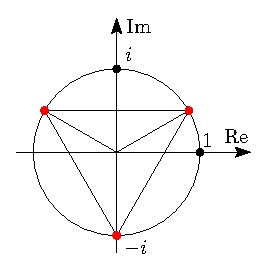
\includegraphics[width=0.3\textwidth]{AL1S3_1.eps}
	\caption{Геометрический поиск корней.}
	\label{AL1S3_1}
\end{figure}

Пусть $w \in \sqrt[n]{z}$, тогда нужно домножить $w$ на числа с аргументами $\tfrac{2\pi k}{n}$, которые будут в множестве: 
$$
	\left\{\cos\tfrac{2\pi k}{n} + i \sin \tfrac{2\pi k}{n} \Big\vert k =0,1\dotsc, n-1\right\} = \sqrt[n]{1} 
$$
$$
	w = \sqrt[n]{R}\left(\cos\tfrac{\alpha }{n} + i \sin \tfrac{\alpha k}{n}\right) \Rightarrow w{\cdot}\left(\cos\tfrac{2\pi k}{n} + i \sin \tfrac{2\pi k}{n}\right) = \sqrt[n]{R}\left(\cos\tfrac{\alpha + 2\pi k}{n} + i \sin \tfrac{\alpha + 2\pi k}{n}\right)
$$
где последнее верно в силу того, что при перемножении комплексных чисел их аргументы складываются. Следовательно:
$$
	w \in \sqrt[n]{z} \Rightarrow \sqrt[n]{z} = w{\cdot}\sqrt[n]{1}
$$
Таким образом, умножить на $n$-ый корень из единицы $\Leftrightarrow$ отложить вершины правильного $n$-угольника.

\begin{problem}(\textbf{К22.7})
	
	л) $\sqrt[6]{-27}$
\end{problem}
\begin{proof}
	$\sqrt[6]{-27} = \left\{\sqrt{3}\left( \cos\tfrac{\pi + 2\pi k}{6} + i\sin \tfrac{\pi + 2\pi k}{6}\right) \Big\vert k = 0,1,\dotsc, 5\right\}$. Геометрически это будет правильный $6$-угольник у которого две вершины будут равны $\pm i\sqrt{3}$.
\end{proof}

\begin{problem}(\textbf{К22.7})
	
	м) $\sqrt[4]{8\sqrt{3}i - 8}$
\end{problem}
\begin{proof}
	$$
		R = |8\sqrt{3}i - 8| = 8|\sqrt{3}i - 1| = 4^2 = 2^4 \Rightarrow \sqrt[4]{R} = 2, \, 8\sqrt{3}i - 8 = 16\left(\tfrac{\sqrt{3}}{2}i - \tfrac{1}{2}\right) \Rightarrow \varphi = \tfrac{2 \pi}{3} \Rightarrow
	$$
	$$
		\Rightarrow \sqrt[4]{8\sqrt{3}i - 8} = \left\{2 \left(\cos\tfrac{\pi + 3\pi k}{6} + i \sin\tfrac{\pi + 3\pi k}{6} \right) \Big\vert k = 0,1,2,3\right\}
	$$
\end{proof}

\subsection*{Свойства корней в комплексных числах}

В $\MR$: $\sqrt[n]{ab} = \sqrt[n]{a}{\cdot}\sqrt[n]{b}$, если $n$-чётно, то накладывается ограничение $a,b \geq 0$.

В $\MC$: $\sqrt[n]{zw} =\sqrt[n]{z}{\cdot}\sqrt[n]{w}$ понимается, как равенство множеств. Произведение множеств это множество всевозможных произведений.
\begin{proof}
	Пусть $u \in \sqrt[n]{z}, \, v \in \sqrt[n]{w}$, тогда $uv \in \sqrt[n]{zw}$, где верно:
	$$
		uv\in \sqrt[n]{zw} \Leftrightarrow (uv)^n = u^nw^n = zw
	$$
	$$
		\sqrt[n]{zw} = uv\sqrt[n]{1}, \, \sqrt[n]{z} = u \sqrt[n]{1}, \, \sqrt[n]{w} = v\sqrt[n]{1}
	$$
	Подставляем в $\sqrt[n]{zw} =\sqrt[n]{z}{\cdot}\sqrt[n]{w}$ и получаем, что нам надо доказать $\sqrt[n]{1} = \sqrt[n]{1}{\cdot}\sqrt[n]{1}$. Введем обозначение:
	$$
		\VE_n = \cos\tfrac{2\pi}{n} + i \sin\tfrac{2\pi}{n} \Rightarrow \sqrt[n]{1} = \left\{1 ,\VE_n, \VE_n^2,\dotsc, \VE_n^{n-1} \right\} = \{\VE_n^k \mid k \in \MZ \}
	$$
	$$
		\forall k,l \in \MZ, \, \VE_n^k{\cdot}\VE_n^l = \VE_n^{k + l} = \VE_n^{k + l \; (\bmod n)} \Rightarrow \sqrt[n]{1}\sqrt[n]{1} \subset \sqrt[n]{1}
	$$
	$$
		\forall k \in \MZ, \, \VE_n^k = \VE_n^k{\cdot}1 \Rightarrow \sqrt[n]{1} \subset \sqrt[n]{1}\sqrt[n]{1}
	$$
\end{proof}
Говорят, что множество: $\left\{1 ,\VE_n, \VE_n^2,\dotsc, \VE_n^{n-1} \right\} = \{\VE_n^k \mid k \in \MZ \}$ \uwave{замкнуто относительно умножения}. По сути оно является группой по умножению: содержит единицу и для любого элемента есть обратный: 
$$
	\forall k \in \MZ, \, (\VE_n^k)^{-1} = \VE_n^{-k}, \, \VE_n^k{\cdot} \VE_n^{-k} =  \VE_n^{k - k} = \VE_n^0 = 1
$$ 
Геометрически, $\VE_n^{-k}$ находится под $\VE_n^k$, то есть это тоже самое, что и комплексно сопряженное число.

Если два комплексных числа в произведении дают единицу, значит их аргументы противоположны. В нашем случае, поскольку модули у чисел равны единице, то они лежат на одной окружности.
$$
	z^{-1} = \ovl{z} \Leftrightarrow |z| = 1
$$
\textbf{Вывод}: для единичной окружности обратное число на ней совпадает с его сопряженным.

\begin{figure}[H]
	\centering
	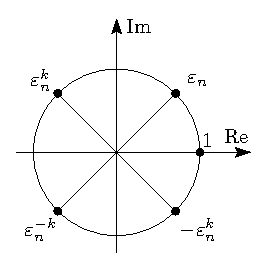
\includegraphics[width=0.3\textwidth]{AL1S3_2.eps}
	\caption{Корни из единицы.}
	\label{AL1S3_2}
\end{figure}

\begin{problem}\hfill	
	\begin{enumerate}[label=\alph*)]
		\item Пусть $z \in \MC, \, |z| = 2$, с помощью циркуля и линейки построить числа: $\dfrac{1}{z},\,  \dfrac{2}{\ovl{z}}$;
		\item Пусть $z \in \MC, \, |z| = 1$, с помощью циркуля и линейки построить числа: $iz$, $(1 + i)z$;
	\end{enumerate}
\end{problem}
\begin{proof}\hfill\\
	$|z| = 2 \Rightarrow \dfrac{1}{z} = \dfrac{\ovl{z}}{|z|^2} = \dfrac{1}{4}\ovl{z} \Rightarrow$ длина уменьшится в $4$ раза и число будет отражено по реальной оси.
	
	$\dfrac{2}{\ovl{z}} = \dfrac{2z}{|z|^2} = \dfrac{1}{2}z \Rightarrow $ длина уменьшится в $2$ раза и число будет на единичной окружности.
	\begin{figure}[H]
		\begin{subfigure}{.5\textwidth}
			\centering
			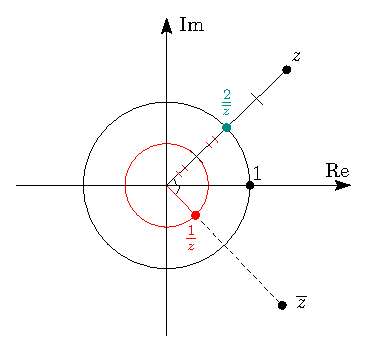
\includegraphics[width=0.6\textwidth]{AL1S3_3.eps}
			\caption{Построение $\tfrac{1}{z}$ и $\tfrac{2}{\ovl{z}}$.}
			\label{AL1S3_3}
		\end{subfigure}
		\begin{subfigure}{.5\textwidth}
			\centering
			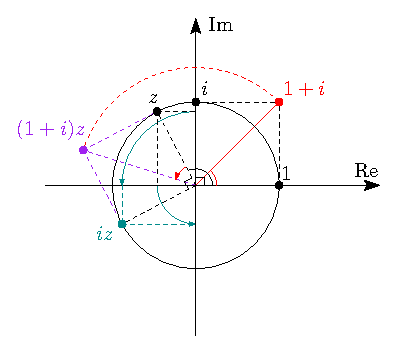
\includegraphics[width=0.7\textwidth]{AL1S3_4.eps}
			\caption{Построение $iz$ и $(1 + i)z$.}
			\label{AL1S3_3}
		\end{subfigure}
	\end{figure}
	Равенство с домножением на сопряженные можно компактно записывать так:
	$$
		z\ovl{z} = |z|^2 \Rightarrow \ovl{z} = \dfrac{|z|^2}{z}, \, \dfrac{1}{z} = \dfrac{\ovl{z}}{|z|^2}
	$$
	Для $z$ поворт на $90^\circ$ это $iz$: $z = a + ib \in \MZ \Rightarrow iz = ia + i^2b = ia - b=  -b + ia$.
	
	$|1+ i| = \sqrt{2}, \, \arg( 1 + i) = \dfrac{\pi}{4} \Rightarrow$ поворот на $45^\circ$ и гомотетия: $|(1 + i)z| = |1 + i|{\cdot}|z| =\sqrt{2}{\cdot}1 = \sqrt{2}$. Но можно сделать попроще: $(1 + i)z = z + iz \Rightarrow$ просто векторное сложение.
\end{proof}

Рассмотрим два корня на единичной окружности: $\sqrt{z}$ и $\sqrt[4]{z^2}$, сколько у них будет значений? У первого будет $2$ корня, у второго $4$. При этом: 
$$
	\sqrt{z}\subset \sqrt[4]{z^2} \subset \MU = \{ z \mid |z| = 1\}
$$
$$
	w \in \sqrt{z} \Rightarrow w^2 = z \Rightarrow  w^4 = z^2 \Rightarrow w \in \sqrt[4]{z}
$$ 
Геометрически, если $z$ лежит на единичной окружности, то чтобы получить его корень, надо поделить угол пополам и прибавить $\pi$, чтобы получить второй угол. 

Когда есть корень $4$-ой степени, значит значения лежат в вершинах квадрата. Две симметричные вершины уже построили, поэтому для получения всех корней $\sqrt[4]{z^2}$ строим перпендикуляр к прямой соединяющей предыдущие два корня и строим правильный квадрат.

\begin{figure}[H]
	\centering
	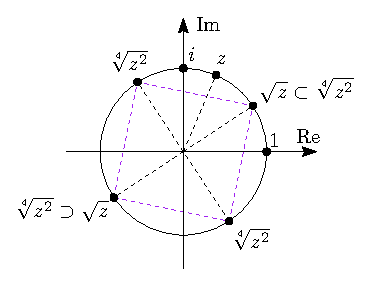
\includegraphics[width=0.35\textwidth]{AL1S3_5.eps}
	\caption{Сравнение корней: $\sqrt{z}$ и $\sqrt[4]{z^2}$.}
	\label{AL1S3_5}
\end{figure}
\begin{problem}
	Изобразить множество корней $\sqrt[8]{1} \setminus \sqrt[4]{1}$.
\end{problem}
\begin{proof}
	На рисунке множество требуемых корней изображено красными точками. Один из корней в алгебраической форме: $\tfrac{1}{\sqrt{2}} + i\tfrac{1}{\sqrt{2}}$.
	\begin{figure}[H]
		\centering
		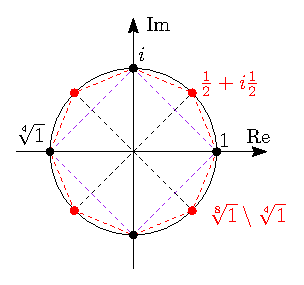
\includegraphics[width=0.3\textwidth]{AL1S3_6.eps}
		\caption{Множество корней: $\sqrt[8]{1} \setminus \sqrt[4]{1}$.}
		\label{AL1S3_6}
	\end{figure}
\end{proof}

\begin{problem}(\textbf{К21.10})
	Если $z + z^{-1} = 2\cos\varphi$, тогда $z^n + z^{-n} = 2\cos (n \varphi)$.
\end{problem}
\begin{proof}
	$$
		z + z^{-1} = 2\cos\varphi \Leftrightarrow z^2 - 2\cos\varphi + 1 =  0 \Rightarrow  z^2 - 2\cos\varphi + 1 = (z - \cos\varphi)^2  + \sin^2\varphi  = 
	$$
	$$
		= (z - \cos\varphi - i\sin\varphi)(z - \cos\varphi + i\sin\varphi) = 0 \Rightarrow z = \cos\varphi \pm i\sin\varphi \Rightarrow
	$$
	$$
		\Rightarrow z^n = \cos(n\varphi) \pm i\sin(n\varphi), \, z^{-n} = \cos(n\varphi) \mp i\sin(n\varphi) \Rightarrow z^n + z^{-n} = 2\cos(n\varphi)
	$$
\end{proof}

\begin{problem}(\textbf{К21.1 x) })
	$1 + \cos\varphi + i \sin\varphi, \, \varphi \in (-\pi,\pi)$.
\end{problem}
\begin{proof}
	$$
		z = 1 + \cos\varphi + i \sin\varphi \Rightarrow |z| = \sqrt{(1 + \cos\varphi)^2 + \sin^2\varphi} = \sqrt{2  + 2\cos\varphi}
	$$
	$$
		1 + \cos\varphi = 2\cos^2\tfrac{\varphi}{2}, \, \varphi \in (-\pi,\pi) \Rightarrow \tfrac{\varphi}{2} \in \left(-\tfrac{\pi}{2}, \tfrac{\pi}{2}\right) \Rightarrow
	$$
	$$
		\Rightarrow \arg{z}  = \alpha \Rightarrow \tg\alpha = \dfrac{\sin\varphi}{1 + \cos\varphi} = \dfrac{2\sin\tfrac{\varphi}{2}\cos\tfrac{\varphi}{2}}{2\cos^2\tfrac{\varphi}{2}} = \tg\tfrac{\varphi}{2} \Rightarrow \alpha = \tfrac{\varphi}{2}
	$$
	$$
		\Rightarrow \sqrt{2  + 2\cos\varphi} = 2\cos\tfrac{\varphi}{2} > 0 \Rightarrow z = 2\cos\tfrac{\varphi}{2}\left(\cos\tfrac{\varphi}{2} + i\sin\tfrac{\varphi}{2}\right)
	$$
	Как можно было сделать представление по-другому? Например, через сложение векторов на единичной окружностия:
	\begin{figure}[H]
		\centering
		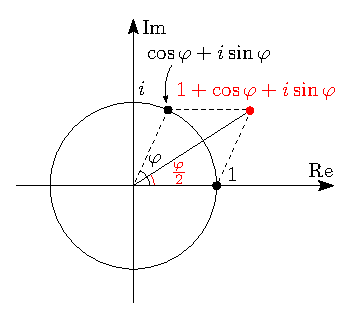
\includegraphics[width=0.35\textwidth]{AL1S3_7.eps}
		\caption{Представление числа: $z = 1 + \cos\varphi + i \sin\varphi$.}
		\label{AL1S3_7}
	\end{figure}
 	Поскольку стороны равны, то мы получаем ромб и его диагональ это биссектрисса угла $\Rightarrow \arg z= \tfrac{\varphi}{2}$.
\end{proof}

\begin{problem}
	$\sqrt[5]{1} = \{1, \VE,\VE^2, \VE^3, \VE^4\}$. Как вычислить $\cos\tfrac{2\pi}{5}, \, \sin\tfrac{2\pi}{5}$?
\end{problem}
\begin{proof}
	$$
		\VE  = \VE_5 = \cos\tfrac{2\pi}{5} + i\sin\tfrac{2\pi}{5}
	$$
	Ключевая идея:
	$$
		1 + \VE + \VE^2 + \VE^3 + \VE^4 =0
	$$
	\uline{Геометрическое объяснение}: Пусть эта сумма не ноль, а какой-то вектор, повернем его на угол $\tfrac{2\pi}{5}$, тогда все векторы перейдут друг в друга $\Rightarrow$ их сумма должна перейти в себя. С другой стороны, если все векторы повернулись на один угол, то их сумма повернулась на тот же угол $\Rightarrow$ противоречие.
	
	\uline{Алгебраическое объяснение}: Можно увидеть из суммы геометрической прогрессии:
	$$
		(1 - \VE)(1 + \VE + \VE^2 + \VE^3 + \VE^4) = 1- \VE^5 = 0, \, 1 -\VE \neq 0 \Rightarrow 1 + \VE + \VE^2 + \VE^3 + \VE^4 = 0
	$$
	И тут можно заметить, что оно связано с геометрическим, поскольку уменожение на $1$ ничего не дает, а умножение на $\VE$ делает сдвиг на $\tfrac{2\pi}{5}$.
	
	\uline{Теорема Виета}: Поскольку мы суммируем корни двучлена: $x^5-1$, то их сумма равна коэффициенту при одночлене $x^4$, то есть равна $0$: $x^5 + 0{\cdot}x^4 + 0{\cdot}x^3 + 0{\cdot}x^2 + 0{\cdot}x - 1$.
	
	Итого, поскольку сумма чисел из $\MC$ равна $0$, то и сумма их действительных частей равна $0$: сумма векторов равна $0 \Rightarrow$ сумма их проекций на любую ось равна $0$, в частности на ось $\RE$, тогда:
	$$
		\RE(1 + \VE + \VE^2 + \VE^3 + \VE^4) = 1 + \cos\tfrac{2\varphi}{5} + \cos\tfrac{4\pi}{5} + \cos\tfrac{4\pi}{5}  + \cos\tfrac{2\varphi}{5} = 0 \Rightarrow 
	$$
	$$
		\Rightarrow 1 + 2\cos\tfrac{2\pi}{5} + 2\cos\tfrac{4\pi}{5} = 1 + 2c + 2(2c^2 - 1) = 0 \Rightarrow 
	$$
	$$
		\Rightarrow 4c^2 + 2x - 1 = 0\Rightarrow c = \dfrac{-1 \pm \sqrt{5}}{4} > 0 \Rightarrow c = \dfrac{-1 + \sqrt{5}}{4} = \cos\tfrac{2\pi}{5}
	$$
	А если бы мы обозначили за $c = \cos\tfrac{4\pi}{5}$, то было бы верно: $\cos\tfrac{2\pi}{5} = \cos\tfrac{8\pi}{5} = 2c^2 -1$ и мы бы получили тот же результат, но:
	$$
		c = \dfrac{-1 \pm \sqrt{5}}{4} < 0 \Rightarrow c = \dfrac{-1 - \sqrt{5}}{4} = \cos\tfrac{4\pi}{5}
	$$	
\end{proof}
\begin{rem}
	Заметим также, что $\cos\tfrac{4\pi}{5}$ получается преобразованием в число золотого сечения (взять с обратным знаком и умножить на $2$).
\end{rem}

\section*{Биномиальные коэффициенты}

Известна формула бинома Ньютона:
$$
	(1 + x)^n = \ddsum{k = 0}{n}C_n^kx^k, \quad C_n^k = \dfrac{n!}{k!(n-k)!}
$$ 
Как найти сумму всех коэффициентов? 
\begin{problem}
	Чему равна сумма:
	$$
		C_n^0 + C_n^1 + C_n^2 + \dotsc + C_n^n
	$$
\end{problem}
\begin{proof}
	Подставим в биноме Ньютона вместо $x$ единицу, тогда:
	$$
		C_n^0 + C_n^1 + C_n^2 + \dotsc + C_n^n = (1 + 1)^n = 2^n
	$$
\end{proof}

Все биномиальные коэффициенты можно увидеть в треугольнике Паскаля:
$$
	\begin{matrix}
		&&&&&&&1&&&&&&\\
		&&&&&&1&&1&&&&&\\
		&&&&&1&&2&&1&&&&\\
		&&&&1&&3&&3&&1&&&\\
		&&&1&&4&&6&&4&&1&&\\
		&&1&&5&&10&&10&&5&&1&\\
		&1&&6&&15&&20&&15&&6&&1
	\end{matrix}
$$
Такое возможно благодаря следующему тождеству:
\begin{prop}
	$$
		C_{n+1}^k = C_{n}^k + C_n^{k-1}, \quad \forall n \in \MN, \, C_n^0 = C_n^n = 1
	$$
\end{prop}
\begin{proof}
	Это тождество можно проверить через факториалы, но можно и исходя из комбинаторной логики, поскольку $C_n^k$ означает количество способов выбрать $k$ элементов из $n$: пусть у нас $n+1$ шар, один из которых черный, остальные - белые. Любое сочетание может либо включать черный шар, либо не включать, если оно не включает, то нам надо выбрать $k$ белых шаров, если же включает, то надо выбрать $k-1$ белый шар.
\end{proof}

\begin{problem}
	Чему равна знакопеременная сумма:
	$$
		C_n^0 - C_n^1 + C_n^2 - \dotsc + (-1)^nC_n^n
	$$
\end{problem}
\begin{proof}
	Аналогично нашему первому вопросу, возникает вопрос 
	$$
		C_n^0 - C_n^1 + C_n^2 - \dotsc + (-1)^nC_n^n = (1 - 1)^n = 0
	$$
\end{proof}

Таким образом, мы можем эти суммы сложить и вычесть. Получим в результате:
$$
	C_n^0 + C_n^2 + C_n^4 + \dotsc  = C_n^1 + C_n^3 + \dotsc = 2^{n-1}
$$
Комбинаторный смысл этого заключается в том, что в $n$-элементном множестве подмножеств из четного числа элементов и из нечётного поровну (всего подмножеств в $n$-элементном множестве равно $2^n$).

\begin{problem}
	Чему равна сумма с шагом $3$:
	$$
		C_n^0 + C_n^3 + C_n^6 + \dotsc
	$$
\end{problem}
\begin{proof}
	Докажем, что верна следующая формула:
	$$
		S_0 = C_n^0 + C_n^3 + C_n^6 + \dotsc = \dfrac{2^n}{3} + \dfrac{2}{3}\cos\dfrac{\pi n}{3} \sim \dfrac{2^n}{3}
	$$
	С первого взгляда это не очень очевидно, как можно сделать. Заметим, что $1$ это корень $1$-ой степени из единицы, $-1$ это корень $2$-ой степени из единицы, теперь (когда берём с шагом $3$) будем подставлять корень $3$-ьей степени из единицы. Если обозначим все корни: $\sqrt[3]{1} = \{1, \VE, \VE^2\}$, то:
	$$
		( 1 + \VE)^n = C_n^0 + C_n^1 \VE + C_n^2 \VE^2 + C_n^3 + C_n^4\VE + C_n^5 \VE^2 + \dotsc = S_0 + S_1\VE + S_2\VE_2
	$$
	\begin{figure}[H]
		\centering
		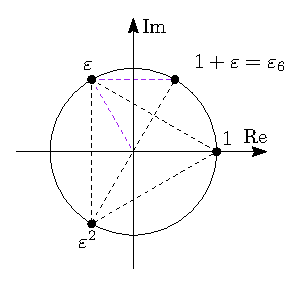
\includegraphics[width=0.25\textwidth]{AL1S3_8.eps}
		\caption{Корень из единицы $3$-ей степени.}
		\label{AL1S3_8}
	\end{figure}
	$$
		\RE(\VE) = \RE(\VE^2) = -\tfrac{1}{2} \Rightarrow \RE((1 + \VE)^n) = S_0 - \tfrac{1}{2}(S_1 + S_2)
	$$
	Также заметим, что $1 + \VE = \VE_6$, для других $n$ так уже могло не получитсься, а здесь получается правильный $6$-угольник. Мы можем воспользоваться формулой Муавра:
	$$
		1 + \VE = \VE_6 \Rightarrow \VE_6^n = (1 + \VE)^n =  \cos\tfrac{\pi n}{3} + i \sin\tfrac{\pi n}{3}
	$$
	Заметим также, что:
	$$
		S_0 + S_1 + S_2 = 2^n \Rightarrow  2S_0  - S_1 - S_2 + S_0 + S_1 + S_2 = 2\cos\tfrac{\pi n}{3} + 2^n \Rightarrow S_0 = \dfrac{2^n}{3} + \dfrac{2}{3}\cos\tfrac{\pi n}{3}  
	$$
\end{proof}
\begin{problem}
	Чему равна сумма с шагом $4$:
	$$
		C_n^0 + C_n^4 + C_n^8 + \dotsc
	$$
\end{problem}
\begin{proof}
	В данном случае в качестве $x$ возьмем $i$, тогда:
	$$
		(1 + i)^n = (C_n^0 + C_n^4 + C_n^8 + \dotsc) + i(C_n^1  + C_n^5 + \dotsc ) - (C_n^2 + C_n^6 + \dotsc ) - i(C_n^3 + C_n^7 + \dotsc ) = 
	$$
	$$
		=S_0 + iS_1 - S_2  - iS_3 \Rightarrow \RE((1 + i)^n) = S_0 - S_2 = 2^{n/2}\cos\tfrac{n \pi}{4}
	$$
	$$
		S_0 + S_2 = C_n^0 +C_n^2 + C_n^4 + \dotsc = 2^{n-1} \Rightarrow 2S_0 = 2^{n-1} + 2^{n/2}\cos\tfrac{n \pi}{4} \Rightarrow 
	$$
	$$	
		\Rightarrow S_0 = 2^{n-2} + 2^{n/2 - 1}\cos\tfrac{n\pi}{4} \sim 2^{n-2} = \dfrac{1}{4}2^n
	$$
\end{proof}
\begin{exrc}
	Доказать, что:
	$$
		C_n^0 + C_n^l + C_n^{2l} + \dotsc \sim \dfrac{1}{l}2^n
	$$
\end{exrc}

\end{document}